\section{Introduction}

A growing body of research uses trait-based approaches to understand how biodiversity links to ecosystem functioning, and how environmental changes are likely to affect species non-randomly with respect to their traits (Hevia et al). Strictly, traits are defined as characteristics measurable the level of an individual, with an effect on organismal fitness or performance. They can be physiological (e.g., metabolic rates), morphological (e.g., body mass), behavioural (e.g., learning) or phenological (e.g., anthesis), or can relate to species life-history (e.g. longevity). This definition can be broadened to include characteristics measurable at the species level, such as the number of habitats known to be used by a species (habitat breadth). Here, I use this broader definition of traits and refer to these as ecological traits.

Many studies have shown that traits influence species responses to environmental pressures (). Moreover, it is now accepted that ecosystem functioning is positively correlated with species functional diversity (Tilman). Species traits can provide a mechanistic understanding of both species roles in ecosystem functioning and of species responses to changes. Traits shape species fundamental and realised niches; for instance, physiological traits influence species thermal tolerances, participating in defining their geographical distributions. Traits such as trophic level or body mass structure food webs and affect inter- and intra-specific competition. As such, traits determine and reflect species use of their environment. Specifically, effect traits define organismal contributions to ecosystem functions. Effect traits are underpinned by species resource use, and this applies at diverse scales, from single-celled nutrient cycling bacteria to large mammals. Response traits are those involved in determining species responses to environmental changes and can overlap with effect traits. 

Although terrestrial vertebrates have been extensively studied in the past (Titley et al), the vast majority of research investigating the impact of environmental changes on ecosystem functions has focused on plants and invertebrates (Hevia et al). Vertebrates nevertheless play diverse ecosystem roles, and some are important keystone species.  Vertebrate species particularly contribute in food web structures and population dynamics through predatory and herbivory activity. They are pollinators and seed dispersers, and overall participate in nutrient cycling at higher levels. Understanding how environmental changes may affect their ecological roles is important to predict future ecosystem functioning, and to put into place appropriate mitigation measures. The end-goals of my PhD thesis are to elucidate how species traits influence their responses to land-use and climate change, and how this links to changes in ecosystem functioning. Addressing these questions requires to use extensive trait data. Despite vertebrates having been the focus of much research, and despite the growing interest for trait-based approaches, there exist no comprehensive database of vertebrate ecological traits encompassing all classes. Consequently, collating trait data was a prerequisite for any further work, and this operation was constrained by the amount of information available in the literature. The present chapter focuses on data collection methods and missing trait values imputations. Thanks to past and recent efforts to release data in the public domain, at least four comprehensive ecological trait databases are now freely accessible (mammals: Pantheria, amphibians: Amphibio, amniotes: Myhrvold, mammals and birds: Cooke et al). Other trait datasets have been released on online platforms alongside published articles (e.g. Global Assessment of Reptile Distribution initiative, \url{http://www.gardinitiative.org/}), or can be downloaded from online databases (IUCN Red List (\url{https://www.iucnredlist.org/}), BirdLife data zone (\url(http://datazone.birdlife.org/home)). Trait data available from primary sources for mammals and birds is likely to be more abundant and more resolved than for reptiles and amphibians, due to systematic biases in sampling with regards to taxonomic groups (Newbold, \textit{manuscript}).

The present chapter details the methodology I employed to collate trait information across terrestrial vertebrates. Primary sources offered a variety of traits, of which only a few were selected. Trait selection was motivated by two main reasons: (1) traits should be of ecological interest and be related to response or effect processes; (2) trait values should be available for many species, across the four terrestrial vertebrate classes, allowing for cross-classes comparative analyses. The selected target traits related to species life-history and morphology (body mass; longevity; litter/clutch size; diel activity; trophic level; diet) and to their habitat preferences (habitat breadth and specialisation). Reptilian diet was not readily available in primary data sources, and one exception was made as I extracted diet data for the other classes. Species mobility was hardly available across sources, and no similar variable could describe species mobility across classes; although species' abilities to move in their environment is likely to strongly impact their responses to threats, this trait was not considered for the above reasons. 

The present chapter details the methodology I employed to collate selected traits. I elaborate on some of the challenges met when compiling data across many species, such as inconsistency of taxonomy across sources. Not unexpectedly, the amount of missing values was highly variable across classes and traits. To achieve full trait coverage across species, I imputed missing trait values using random-forest algorithms.
In this chapter, I briefly examine imputation performance, notably by assessing whether increasing species representation in phylogenetic trees affects imputation error. 

In October 2018, Cooke et al released a comprehensive database of six mammalian and avian traits. They collated and imputed missing trait values for body mass, litter/clutch size, volancy, diel activity, primary diet and habitat breadth. As similar primary sources were used in both our data collection, I did not use their database to complement my sources. Moreover, the imputation methods they used to fill gaps in trait coverage differed from mine. I used this freely accessible compiled data as an opportunity to compare the results of both our data collection and imputation processes. This chapter also presents results from this comparison (more extensively so in the SI).

Finally, the trait data collected and imputed in this chapter can be subject to future changes, and may not final at this stage.

%Finally, I briefly examine patterns in missing values with regards to species phylogenetic position.




\pagebreak
\section{Methods}

\subsection{Ecological trait data collection}

\subsubsection{Primary data sources.}
I collated ecological trait data for terrestrial vertebrates from the sources figuring in Table \ref{datasources}. Information was compiled for the following target traits: body mass, longevity, litter or clutch size, trophic level, diel activity, diet, and habitat preferences. I also compiled traits that were potentially correlated to either body mass or longevity, to be used as potential predictors in imputations of missing values. As such, body length information was compiled when available, as well as generation length or age at sexual maturity. Most notably, longevity was chosen over generation length or age at sexual maturity as it was the only common currency across classes reflecting generation turnover. In addition, species geographical range sizes were estimated from distribution data, extracted from the IUCN Red List.

% Table of sources.
\begin{table}[h!]
\renewcommand{\baselinestretch}{1}
\renewcommand{\arraystretch}{1.5}
\begin{center}\fontsize{9}{11}\selectfont
\caption[Primary sources used for each compiled trait.]{\textbf{Primary sources used for each compiled trait.} Primary sources may contain more traits than shown here. \textbf{BM}: body mass; \textbf{BL}: body length; \textbf{L}: longevity or maximum longevity; \textbf{GL}: generation length; \textbf{LCS}: litter or clutch size; \textbf{TL}: trophic level; \textbf{Di}: diet; \textbf{DA}: diel activity; \textbf{RS}: range size; \textbf{H}: habitat data. Bolded abbreviations highlight target traits; other traits were added for potential correlations in further imputations.} 
\label{datasources}
\begin{tabular}{|l|c|c|c|c|c|c|c|c|c|c|c|c|}
\hline
\multicolumn{1}{|c|}{\multirow{2}{*}{\textbf{Sources}}} & \multirow{2}{*}{\textbf{Taxa}} & \multicolumn{9}{c|}{\textbf{Traits}} & \multirow{2}{*}{\textbf{RS}} & \multirow{2}{*}{\textbf{H}} \\ \cline{3-11}
\multicolumn{1}{|c|}{} &  & \textbf{BM} & BL & \textbf{L} & MA & GL & \textbf{LCS} & \textbf{TL} & \textbf{Di} & \textbf{DA} &  &  \\ \hline
Amphibio & \multirow{4}{*}{Amphibians} & \checkmark & \checkmark & \checkmark & \checkmark &  & \checkmark & \checkmark & \checkmark & \checkmark &  &  \\ \cline{1-1} \cline{3-13} 
Cooper &  &  & \checkmark &  &  &  & \checkmark &  &  &  & \checkmark &  \\ \cline{1-1} \cline{3-13} 
Senior &  &  & \checkmark &  &  &  &  &  &  &  &  &  \\ \cline{1-1} \cline{3-13} 
Bickford &  &  & \checkmark &  &  &  &  &  &  &  & \checkmark &  \\ \hline
Elton & \multirow{2}{*}{Birds} & \checkmark &  &  &  &  &  &  & \checkmark & \checkmark &  &  \\ \cline{1-1} \cline{3-13} 
Butchart &  & \checkmark &  &  &  & \checkmark &  &  &  &  &  &  \\ \hline
Pantheria & \multirow{5}{*}{Mammals} & \checkmark & \checkmark & \checkmark & \checkmark &  & \checkmark &  &  & \checkmark &  &  \\ \cline{1-1} \cline{3-13} 
Kissling1 &  &  &  &  &  &  &  & \checkmark &  &  &  &  \\ \cline{1-1} \cline{3-13} 
Kissling2 &  &  &  &  &  &  &  & \checkmark &  &  &  &  \\ \cline{1-1} \cline{3-13} 
Elton &  & \checkmark &  &  &  &  &  &  & \checkmark & \checkmark &  &  \\ \cline{1-1} \cline{3-13} 
Pacifici &  & \checkmark &  & \checkmark & \checkmark & \checkmark &  &  &  &  &  &  \\ \hline
Scharf & \multirow{8}{*}{Reptiles} & \checkmark &  & \checkmark & \checkmark &  & \checkmark & \checkmark &  & \checkmark &  &  \\ \cline{1-1} \cline{3-13} 
%Meiri &  &  &  &  &  &  &  & \checkmark &  & \checkmark &  &  \\ \cline{1-1} \cline{3-13} 
Vidan &  &  &  &  &  &  &  &  &  & \checkmark &  &  \\ \cline{1-1} \cline{3-13} 
Stark &  & \checkmark &  & \checkmark &  &  & \checkmark &  &  & \checkmark &  &  \\ \cline{1-1} \cline{3-13} 
Schwarz &  &  &  &  &  &  & \checkmark &  &  &  &  &  \\ \cline{1-1} \cline{3-13} 
Novosolov1 &  & \checkmark &  &  &  &  &  & \checkmark &  &  & \checkmark &  \\ \cline{1-1} \cline{3-13} 
Novosolov2 &  &  &  &  &  &  & \checkmark &  &  &  &  &  \\ \cline{1-1} \cline{3-13} 
Slavenko &  & \checkmark &  &  &  &  &  &  &  &  &  &  \\ \hline
Myhrvold & Amniotes & \checkmark & \checkmark & \checkmark & \checkmark &  & \checkmark &  &  &  &  &  \\ \hline
IUCN & Vertebrates &  &  &  &  &  &  &  &  &  & \checkmark & \checkmark \\ \hline
\end{tabular}
\end{center}
\end{table}

\subsubsection{Compilation methods.}

\paragraph{Continuous traits.}
All continuous traits were averaged within species when different sources provided estimates. Longevity and maximum longevity were assumed to provide the same information and were averaged within species. No measure of intra-specific variability was compiled and estimates were provided as a single measure for each species.

\paragraph{Categorical traits.}
\subparagraph{Activity time.}
Species were described as being either nocturnal or non-nocturnal. Despite a higher resolution of activity time information in some of the primary sources (e.g. species being described as cathemereal, crepuscular or strictly diurnal), I adopted the classification of the primary source with the lowest resolution, in order to have consistent information across classes.
\subparagraph{Diet and diet breadth.}
For mammals and birds, diet was compiled from the Elton Traits database (ref). Primary diet was available in the avian dataset and declined into five categories: (1) plant or seed consumers; (2) fruit or nectar consumers; (3) vertebrate consumers, including fish and carrion; (4) invertebrate consumers; and (5) omnivores. Primary diet was not available for mammals. Instead, mammal diet was only described as the percent use of different food items. I pooled these items together into the same five primary diet categories as for the avian dataset. Any food items for which percent use was equal to or above 50\% were considered to be primary food items. Species for which no food item had percent use above 50\% were considered to be omnivores.\\ 
For amphibians, diet information was extracted from AmphiBIO. Diet information was available as binary variables for diverse food items. Percent use were not recorded, so these items were considered to form species primary diet. I pooled amphibian species into the five diet categories described above.
\subparagraph{Trophic level.} For amphibians and birds, trophic levels were partly inferred from the primary diet. 
\subparagraph{Habitat preferences.}
Species habitat preferences were compiled from IUCN habitat data files and were described as a binary variable recording whether a species was known to occur in a particular habitat. I calculated habitat breadth as the number of habitats a species was known to use. Weights were assigned to each habitat in this calculation depending on the recorded habitat suitability and importance; outcomes were not very sensitive to the presence of weights (compared to a non-weighted sum, see SI). Finally, a broad degree of habitat specialisation was produced. If any artificial habitat was recorded to be suitable, species were reported to be generalists; else, they were natural habitat specialists. More details on habitat preferences compilation are provided in the SI. 

\subsection{Phylogenetic information}
I obtained phylogenetic trees for birds, amphibians, mammals and squamates from Hedges et al (2015) (available at \url{http://www.biodiversitycenter.org/ttol}, downloaded 06/07/2018). All trees were ultrametric and fully resolved, except for the amphibian tree which presented polytomies. All trees contained a few branches of length 0 (193 branches for mammals, 136 for amphibians, 189 for birds and 284 for reptiles).

\subsection{Tackling taxonomic synonymy}
Across the different primary sources, similar species could appear under different binomial names. This was a problem when matching datasets by species. It was also problem when matching species to the PREDICTS database. Moreover, it is possible than within a primary source, a given species was appearing under two or more different names. As such, taxonomic synonymy created `pseudoreplicates' of the same species, overall falsely increasing the total number of species and artificially inflating the amount of missing trait values. Taxonomic synonymy was hence a major issue; due to the large number of species across datasets, extensive manual checks could not be applied. The presence of typos in species names had the same effect as synonymy, erroneously duplicating species. I attempted to correct for taxonomy first by correcting for typos, and second by identifying species which were entered under a synonymic name and replacing these with the accepted name. To this end, I developed an automated procedure, complemented with a few manual entries. Obvious cases where vernacular names had been entered in the place of binomial names were also treated manually; that was the case for 44 PREDICTS species (when possible, I best assigned binomial names to species common names; unidentifiable species were left empty and assigned to a genus (5 species)).

\subsubsection{Automated procedure and outputs.}
\paragraph{Extracting names from the IUCN Red List and the Integrated Taxonomic Information System (ITIS).}
The automated procedure consisted in extracting species accepted and synonymic binomial names from the IUCN Red List or from the ITIS, using the rredlist and taxize R packages. I started by generating a list of all names figuring across datasets (primary sources, phylogenies and PREDICTS). These `original' names were corrected for typos; then, the IUCN Red List was queried and synonyms and accepted names were stored when possible. When species were not found in the IUCN Red List, information was extracted from ITIS. When species were not found in ITIS either, corrected names were assumed to be accepted. Family and order information was extracted using the same procedure and some entries were completed using the Global Biodiversity Information Facility taxonomic backbone (\url{https://www.gbif.org/tools/species-lookup}).\\
\textbf{NB:} for species entered with the forms \textit{Genus cf.}, \textit{Genus aff.} or \textit{Genus spp.}, the accepted name was left empty.

\paragraph{Outputs.} I generated a list of vertebrate species, recording whether species names were accepted or synonymic (for 14124, 8743, 6090, and 11183 names or identifiers found across datasets for birds, amphibians, mammals and reptiles respectively, including species names as they appeared in phylogenetic trees). For each name, the identified accepted name and the synonyms were stored when possible, as well as additional taxonomic information (order, family, genus). When queries did not succeed, species accepted names were assumed to be the original names found in the datasets.

\paragraph{Harmonising taxonomy in trait datasets.}
Taxonomy across datasets was finally homogenised by replacing recorded synonyms with their accepted scientific names. Overall, this procedure  reduced the total number of species figuring in trait datasets (Figure \ref{taxcor}). The species presenting the highest degree of pseudoreplication was the East African mole rat (\textit{Tachyoryctes splendens}), which was figuring under 12 names identified as being synonymic across primary sources (Figure \ref{taxcor}B), highlighting the need for normalising taxonomy across sources.

% figure: distribution of names and differences in species number
\vspace{0.5cm}
\begin{figure}[h!]
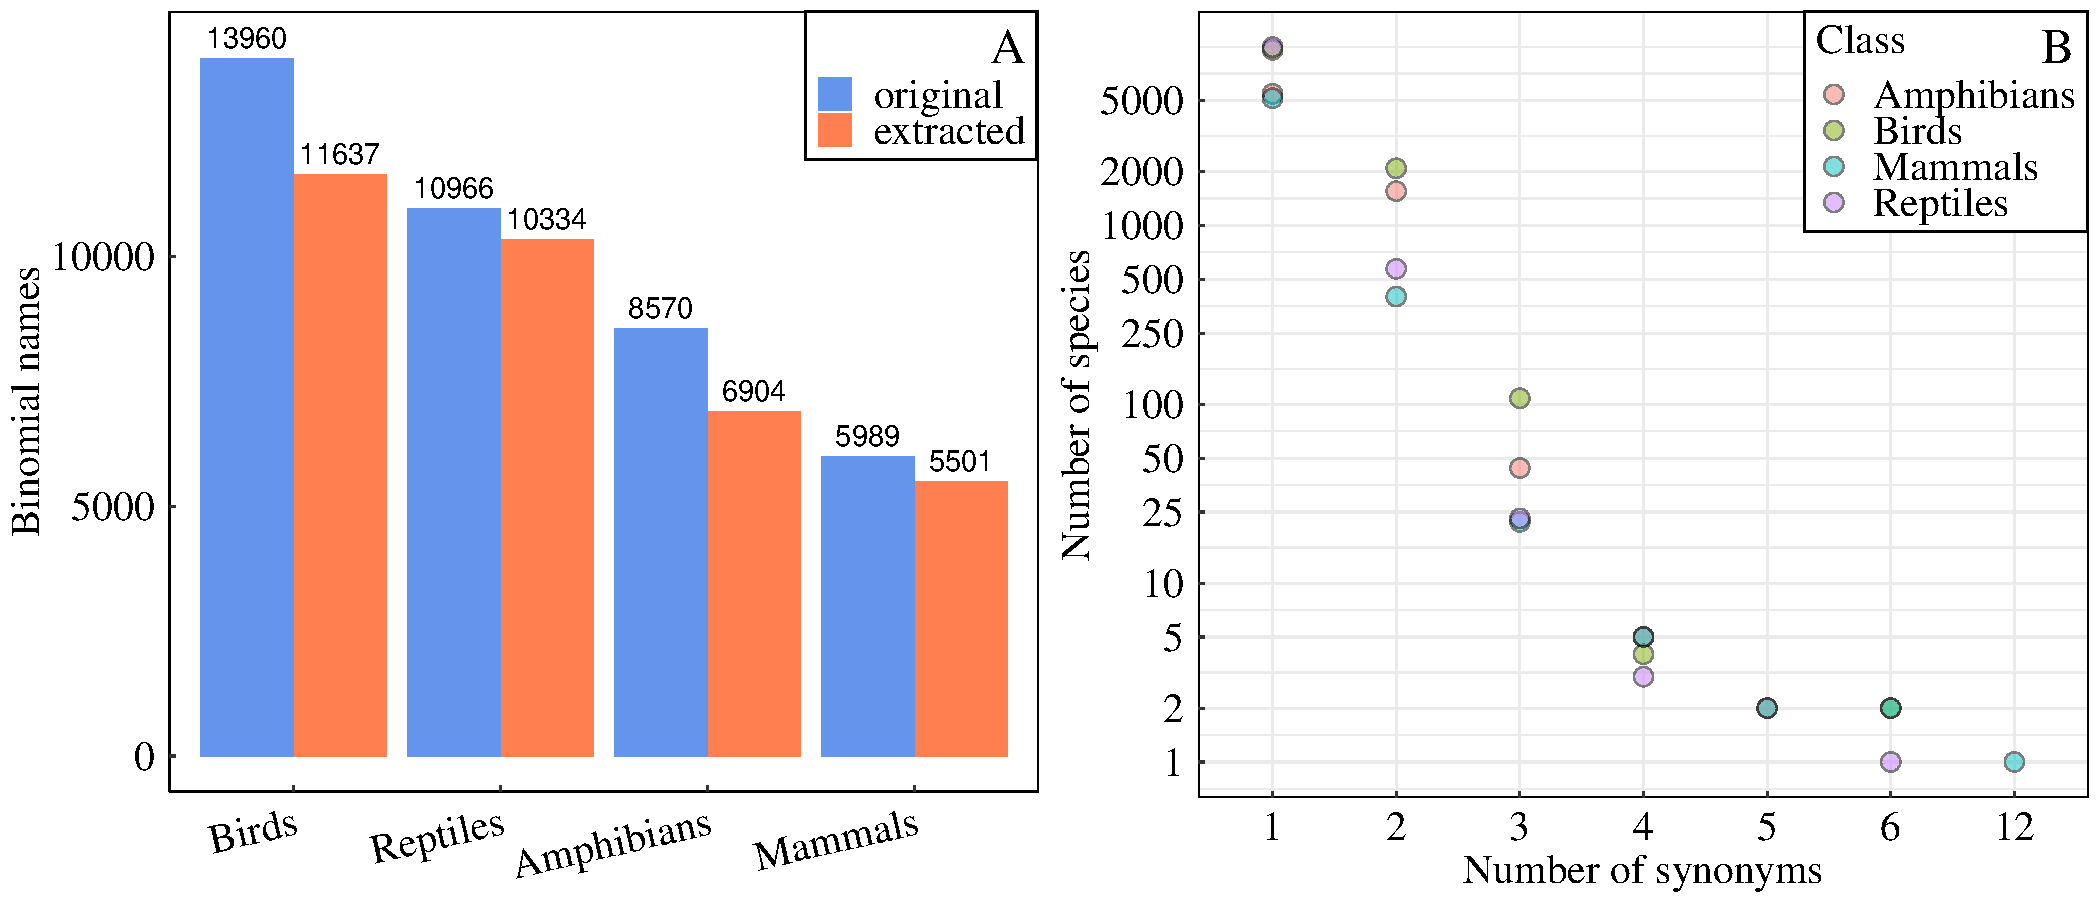
\includegraphics[scale=0.45]{figures/chapter2/Taxonomic_corrections/tax_corrections}
\caption[Difference in species number due to taxonomic correction (A) and distribution of number of synonyms across datasets (B)]{\textbf{Difference in species number due to taxonomic correction (A) and distribution of number of synonyms across datasets (B).} \textbf{(A)} shows the number of species across all primary sources (trait datasets and PREDICTS, excluding phylogenies), before and after correcting for taxonomy. Replacing identified synonyms by the extracted accepted name reduced the number of species in all classes, with the most drastic reduction for birds (decrease by 2,323 unique binomial names). The diminution was of 632 unique identified species for reptiles, of 1,666 for amphibians and of 488 for mammals. \textbf{(B)} shows the distribution of the number of synonymic names. In all four classes, more than 5,000 species (or binomial names) had no identified synonyms. Nevertheless, a large amount of species had two identified synonyms (range: 400 species for mammals - 2086 for birds). The most replicated species was the East African mole rat \textit{Tachyoryctes splendens}, for which 11 synonyms were identified.}
\label{taxcor}
\end{figure}

Despite the automation efforts, taxonomic redundancy persisted to a degree in the trait datasets. Indeed, at this stage, not all species in PREDICTS matched a species in the trait datasets. Additional manual inputs were required to resolve taxonomic synonymy for these species. Verifying the presence of PREDICTS species in trait datasets was important for further analyses. Taxonomic synonymy was resolved manually for 91 PREDICTS species that did not match any species in the trait datasets; in that case, information was extracted from other diverse sources (such as the Reptile Database (\url{http://www.reptile-database.org/}); Avibase (\url{https://avibase.bsc-eoc.org/avibase.jsp?lang=EN&pg=home}); AmphibiaWeb (\url{https://amphibiaweb.org/})). After adding manual inputs to the synonym datasets, all PREDICTS species were represented in trait datasets. 

The need to apply additional manual inputs underlines the fact that the automated procedure was not optimal. The Red List and the ITIS were not comprehensive taxonomic sources, and for clades with high degrees of pseudoreplication in names, such as reptiles or amphibians, neither the Red List or the ITIS were fully resolved. As I only applied manual checks for PREDICTS relevant species, `pseudoreplication' and taxonomic errors are likely to have persisted to a degree. Moreover, certain species were entered using the format \textit{Genus subspecies} rather than \textit{Genus species}; for these, automated queries may have failed to identify the species.

% Extract of synonym dataset? in the SI


\subsubsection{Harmonising taxonomy in phylogenetic trees and increasing species phylogenetic representation.}

\paragraph{Taxonomic correction across tip labels.} 
Efforts to correct datasets for taxonomy created problems for a marginal proportion of species when dealing with phylogenies. The idea of the procedure described above was to replace two or more identified synonyms by a single accepted name, and then collapsing dataset rows together by names. I applied the same method on phylogenies, replacing synonyms by their identified accepted names in trees' tip labels. Not unexpectedly, in some cases, the procedure ended up assigning the same accepted name to different phylogenetic tips. This was the case for 2.8\% of mammalian, 1.7\% of avian, 1.6\% of amphibian and  1.7\% of reptilian species, which then had multiple phylogenetic positions (most having two different positions, see SI). Because keeping several putative phylogenetic positions for a species was problematic in further analyses, I selected one tip to conserve and dropped other tips from the phylogenies (Figure \ref{chart_phylorep}). To briefly describe the procedure, if replicated tips were sister clades, the tip to conserve was chosen randomly among the replicates. Else, I chose to conserve the tree tip whose position was closest to the position of the same tip in the uncorrected tree, when present. In all other few cases, tips to drop were chosen randomly. Further details on how replicated tips were dropped are available in the SI (with 3 examples for each case of Figure \ref{chart_phylorep}).

\begin{figure}[h!]
\centering
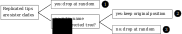
\includegraphics[scale=0.7]{figures/chapter2/chart_phylorep}
\caption[Procedure followed to drop replicated tips from phylogenies]{\textbf{Procedure followed to drop replicated tips from phylogenies.} Most of these were replicated twice. When replicated tips were sister clades, the tips to drop were chosen randomly, as it did not affect the `true' phylogenetic position of the species (1). When replicated were not sister clades, I kept the tip whose position was closest to the position of the same tip in the uncorrected tree (2). In a few cases, the corrected name did not appear in the original tree. Those were problematic cases, and the tips to drop were chosen randomly (3). Nevertheless, occurences of that third case were rare (see SI).}
\label{chart_phylorep}
\end{figure}

\begin{figure}[h!]
\centering
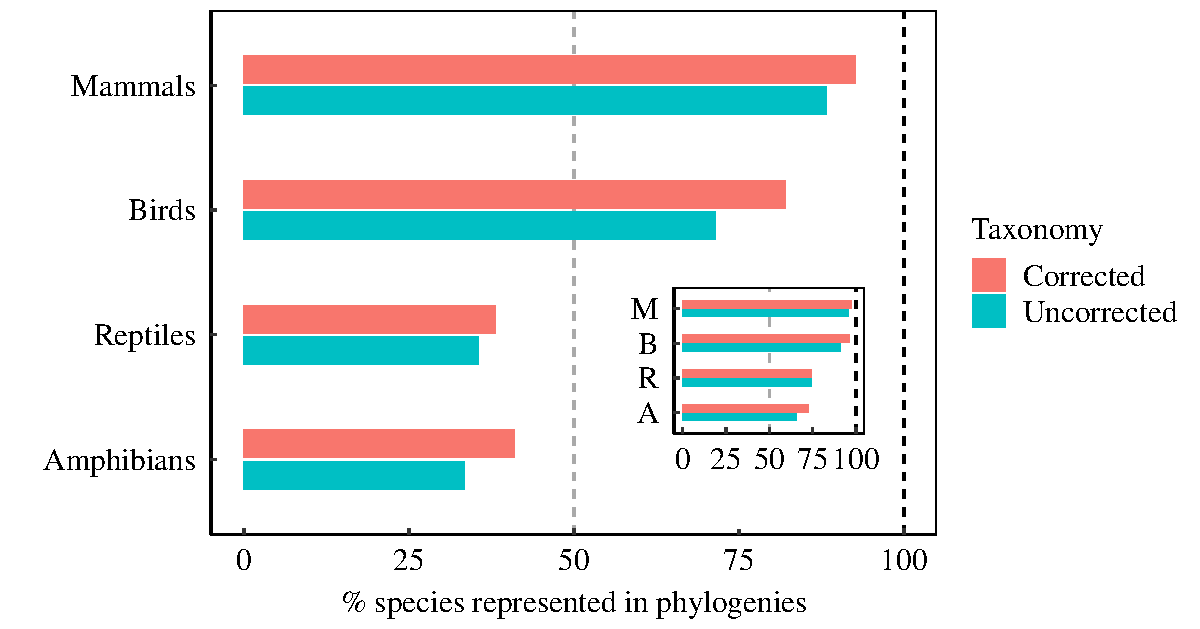
\includegraphics[scale=0.7]{figures/chapter2/Species_representation_phylo}
\caption[Percentage of species represented in the phylogenies for both corrected and uncorrected trait datasets]{\textbf{Percentage of species represented in the phylogenies for both corrected and uncorrected trait datasets.} Overall, taxonomic correction increased species representation in phylogenetic trees. Representation for mammals and birds was high (after taxonomic correction: 82\% of avian and 93\% of mammalian species had a phylogenetic position). On the other hand, reptiles and amphibians were poorly represented (after taxonomic correction: only 38\% of reptilian and 41\% of amphibian species were placed in phylogenetic trees). The inset barplot shows representation for species figuring in PREDICTS. For these, species presence in phylogenetic trees after correction was high across all classes, with a minimum representation of 76\% for amphibians.}
\label{species_rep_phylo}
\end{figure}

\paragraph{Correcting for taxonomy in the phylogenies: conclusions.}
Overall, correcting for taxonomy in phylogenies improved species representation in the trees (Figure \ref{species_rep_phylo}. For amphibian and reptilian species figuring in PREDICTS only, phylogenetic representation disproportionally increased (with a minimum representation of 76\% for PREDICTS amphibians after correcting the trees for taxonomy, inset plot in Figure \ref{species_rep_phylo}). Nevertheless, correcting phylogenetic tip labels generated replicates for a marginal number of tips, which then had to be dropped. 


\paragraph{Species attachments to phylogenetic trees.} Some species in the trait datasets were not represented in the phylogenies. Maximising the number of species represented in the phylogenies was important for further trait imputations. Indeed, if traits were evolutionary conserved, species phylogenetic position could be an important predictor of trait values. To maximise species representation, I added some species to the root of their genus, when possible (phytools package). Attaching species at the root of their genus created polytomies, which were resolved randomly (using multi2di, ape package). Resulting trees contained branches of length zero. To facilitate further analyses, a small number ($10^{-10}$) was added to these branch lengths; consequently, the trees were not ultrametric.  were Such a process could have altered the significance and the strength of trait phylogenetic signal. I further verify whether these alterations of the trees had impacted phylogenetic signal, by qualitatively comparing the strength and the significance of phylogenetic signal for each trait estimated using both original trees and augmented trees (see `Assessing phylogenetic signal in traits').

A large number of species were attached to their genera in the trees (Table \ref{random_attachments_phy}); for instance, only 38\% of the species figuring in the reptilian trait dataset were initially found in the squamate phylogeny. After attaching non-represented species, 91\% of the species were placed in the squamate phylogeny. 

\begin{table}[h!]
\renewcommand{\baselinestretch}{1}
\renewcommand{\arraystretch}{1.5}
\begin{center}\fontsize{9}{11}\selectfont
\caption[Species representation in phylogenetic trees (corrected taxonomy)]{\textbf{Species representation in phylogenetic trees (corrected for taxonomy).} The number of species attached to the root of their genus ranged from 175 (mammals) to 5438 (reptiles). Finally, most species were represented in the phylogenies, whereas more than half reptilian and amphibian species initially had no known phylogenetic position.} 
\label{random_attachments_phy}
\begin{tabular}{|l|l|l|c|l}
\cline{1-4}
\multicolumn{1}{|c|}{\textbf{Class}} & \multicolumn{1}{c|}{\textbf{Initially not in tree}} & \multicolumn{1}{c|}{\textbf{Of which randomly attached}} & \textbf{No final representation in tree} &  \\ \cline{1-4}
Amphibians                  & 59\% (4040 of 6904)                           & 96\% (3883 of 4040)                     & \textbf{2.3\%}             &  \\ \cline{1-4}
Birds                       & 18\% (2085 of 11637)                          & 75\% (1574 of 2085)                    & \textbf{4.4\%}             &  \\ \cline{1-4}
Mammals                     & 7.4\% (407 of 5502)                           & 43\% (175 of 407)                       & \textbf{4.2\%}            &  \\ \cline{1-4}
Reptiles                    & 62\% (6391 of 10334)                          & 85\% (5438 of 6391)                    & \textbf{9.2\%}             &  \\ \cline{1-4}
\end{tabular}
\end{center}
\end{table}


\subsection{Exploring biases in the coverage and completeness of trait information across classes}
Having normalised taxonomy and compiled trait data, I assessed trait coverage, defined as the percentage of species for which trait information was available for a given trait. To estimate the amount of trait information available for a species, I calculated trait completeness. For a species, trait completeness was defined as the proportion of traits for which information was available (number of non-missing trait values divided by total number of traits). In corrected datasets, species with 0\% completeness in predictor traits were filtered out.

Further, I examined whether patterns in the distribution of missing values emerged within classes, as particular clades or parts of the phylogenies could be under-sampled compared to other clades.
Whether values are missing at random is likely to impact imputation errors, notably if some taxa are under-sampled compared to others. To assess whether missing values presented patterns, I plotted within-family median completeness and coverage values in each branches of phylogenetic trees built at the family level. Tree branches were colour-coded to reflect the median value in each family. Specifically, within family trait completeness was calculated by aggregating species into their families and calculating the median trait completeness within each group. 
Patterns of missing values in trait coverage were explored for each trait separately. Trait coverage was assessed within families as the number of species for which values were missing over total number of species in each family. As families represented by very few species might present higher percentages of missing values, reflecting family size rather than randomness in sampling, I contrasted trait coverage plots against a plot showing how much each family contributed to the total number of species (number of species in each family over total number of species in the tree).


\subsection{Imputing missing trait values}
In order to achieve full trait coverage across classes, I imputed missing trait values. Diverse imputation methods have been developed and used in published articles. Penone et al (2014) assessed the performance of four different imputation approaches (K-nearest neighbour (kNN, Troyanskaya 2001), multivariate imputation by chained equations (mice, van Buuren 2009, 2011), random forest algorithms implemented with missForest (Stekhoven, 2011) and phylogenetic imputations implemented with phylopars (Goolsby, 2016)). Their study showed that the kNN approach resulted in significantly higher imputation errors than the three other approaches. Both missForest and phylopars were the best methods when phylogenetic information was included. Nevertheless, phylopars was much slower than missForest, and could only handle continuous traits. missForest was faster and could deal with mixed type data. Without phylogenetic information, mice was found to be the best method, with fast imputations of mixed-type data. Of all these methods, missForest was the only one that did not make assumptions about data distribution (being a non-parametric approach), or that did not require a prior knowledge of some tuning parameters. As such, missForest appeared to be an interesting option for missing data imputation. To further assess whether to use random forests rather than multivariate chained equations, I estimated the phylogenetic signal in traits. Strong phylogenetic signal in traits would indicate than missForest could perform better than mice.

\subsubsection{Assessing phylogenetic signal in traits}

\paragraph{Measuring phylogenetic signal in continuous traits with Pagel's $\lambda$.}
Phylogenetic signal is a measure of the tendency of closely related species to resemble each other more than less related species. Diverse statistics have been developed to estimate phylogenetic signal, most of them applying to continuous traits (Munkemuller 2012). I used Pagel's $\lambda$ (function phylosig, phytools package). Pagel's $\lambda$ is a scaling component that measures the coefficient by which the trait covariance matrix should be weighted to fit a Brownian motion model of evolution. Indeed, under a Brownian motion model of evolution, the trait covariance matrix is expected to be influenced only by the phylogenetic history: changes in trait values happen at random and trait variance is proportional to evolutionary time. When other factors are at play, the observed covariance matrix is the expected covariance matrix transformed with the estimated $\lambda$. A value close to 0 indicates that the covariance matrix need not be transformed by much to fit a Brownian motion. On the other hand, a value close to 1 indicates that trait values are more similar in closely related species than expected under a Brownian motion model of evolution. Using Pagel's $\lambda$, I assessed the strength of the phylogenetic signal. The phylosig function (phytools) also allows to test for signal significance (comparing the estimated $\lambda$ to the null expectation of $\lambda$ with a log-likelihood ratio test). Note that the function developed by Borges et al does not work if phylogenetic trees contain branches of length 0. As both original and corrected phylogenies contained 0-length branches, I added a very small number to these ($10^{-10}$) to remedy to this issue. As such, the trees with which $\delta$ was computed were not ultrametric. 

\paragraph{Measuring phylogenetic signal in categorical traits with $\delta$ (Borges et al, 2018).}
Very few methods have been developed to measure and test phylogenetic signal in categorical traits. Fritz and Purvis (2010) introduced the $D$-statistic, which only applies to binary traits. Furthermore, $D$ is based on a discretisation of the trait, which behaves as a continuous trait evolving under Brownian motion. Borges et al (2018) introduced a new statistic, $\delta$, to measure phylogenetic signal in categorical traits. $\delta$ is based on Shannon entropy principles and uses Bayesian inferences for estimation. $\delta$ can take any positive number, with higher values indicating stronger signal. To test for the significance of the signal, the authors propose to compare the estimated value with a null distribution of values. I generated null distributions of $\delta$  for each trait by simulating 100 random trait vectors (simulating Brownian motion of trait evolution) and calculating $\delta$ for each. I then calculated the median of simulated $\delta$ values as well as 95\% confidence intervals. I tested whether the null-medians were significantly lower than the observed value of $\delta$ using one-sided Wilcoxon rank sum tests. 


\paragraph{Significant phylogenetic signal in all traits}
All traits showed significant phylogenetic signal (Table \ref{physignal}), although the strength of the signal was 

Despite much variation in sample sizes across classes, results indicated strong phylogenetic signal across both categorical and continuous traits (Table \ref{physignal}). The signals were all significant (expect for amphibian body mass, but the signal in body length was strong and significant in this class). Signal strength was overall higher for mammals and birds, which may be a consequence of missing value biases. p-values outputs of the likehood-ratio tests and the Wilcoxon rank sum tests are provided in the SI.

\begin{table}[h!]
\renewcommand{\baselinestretch}{1}
\renewcommand{\arraystretch}{1.5}
\begin{center}\fontsize{9}{11}\selectfont
\caption[Phylogenetic signal in continuous and categorical traits and in range size]{\textbf{Phylogenetic signal in continuous and categorical traits and in range size.} \textbf{BM}: body mass; \textbf{L}: longevity; \textbf{LCS}: litter/clutch size; \textbf{HB}: habitat breadth; \textbf{DB}: diet breadth; \textbf{GL}: generation length; \textbf{BL}: body length; \textbf{SM}: sexual maturity; \textbf{RS}: range size; \textbf{TL}: trophic level; \textbf{PD}: primary diet; \textbf{DA}: diel activity; \textbf{Sp}: specialisation. The phylogenetic signal in continuous traits was calculated with Pagel's $\lambda$. For categorical traits, the $\delta$ metric developed by Borges et al (2018) was used. A star indicates a significant signal (significant p-values scores for the log-likelihood ratio test in the case of $\lambda$; and significant difference from the simulated null distribution of $\delta$ for categorical traits, see SI). `na' are introduced for traits that were not considered in a class but may have been used in another as a predictor in missing values imputations. All traits showed significant phylogenetic signal, with signals for BM, L, LCS, and GL being particularly strong in mammals and birds (above 0.9). Here all calculations were conducted with the corrected phylogenies, after species additions at the root of their genus. See SI for phylogenetic signals computed with the original phylogenies.} 
\label{physignal}
\begin{tabular}{|l|c|c|c|c|c|c|c|c|c|c|c|c|c|}
\hline
\multicolumn{1}{|c|}{\multirow{2}{*}{\textbf{Class}}} & \multicolumn{9}{c|}{\textbf{\begin{tabular}[c]{@{}c@{}}Continuous target traits,\\ additional predictors and range size: $\lambda$\end{tabular}}} & \multicolumn{4}{c|}{\textbf{\begin{tabular}[c]{@{}c@{}}Categorical traits:\\ $\delta$\end{tabular}}} \\ \cline{2-14} 
\multicolumn{1}{|c|}{}                                & \textbf{BM}    & \textbf{L}   & \textbf{LCS}   & \textbf{HB}   & \textbf{DB}   & \textbf{GL}   & \textbf{BL}   & \textbf{SM}   & \textbf{RS}   & \textbf{TL}           & \textbf{PD}           & \textbf{DA}                & \textbf{Sp}          \\ \hline
\textbf{Mammals}                                      & 1.0*           & 0.97*        & 0.96*          & 0.70*         & 0.99*         & 0.99*         & 1.0*          & na            & 0.99*         & 17*                   & 50*                   & 19*                        & 1.4*                 \\ \hline
\textbf{Birds}                                        & 1.0*           & 0.87*        & 0.92*          & 0.50*         & 0.49*         & 0.99*         & na            & na            & 0.67*         & 10*                   & 18*                   & 28$\cdot$10$^3$*           & 1.6*                 \\ \hline
\textbf{Reptiles}                                     & 0.36*          & 0.81*        & 0.72*          & 0.39*         & na            & na            & 0.98*         & 0.87*         & 0.41*         & 4.3*                  & na                    & 7.1*                       & 1.5*                 \\ \hline
\textbf{Amphibians}                                   & 0.80*          & 0.33*        & 0.63*          & 0.77*         & 0.71*         & na            & 0.96*         & na            & 0.54*         & 18*                   & 3.7*                  & 2.9*                       & 3.6*                 \\ \hline
\end{tabular}
\end{center}
\end{table}

\begin{figure}[h!]
\centering
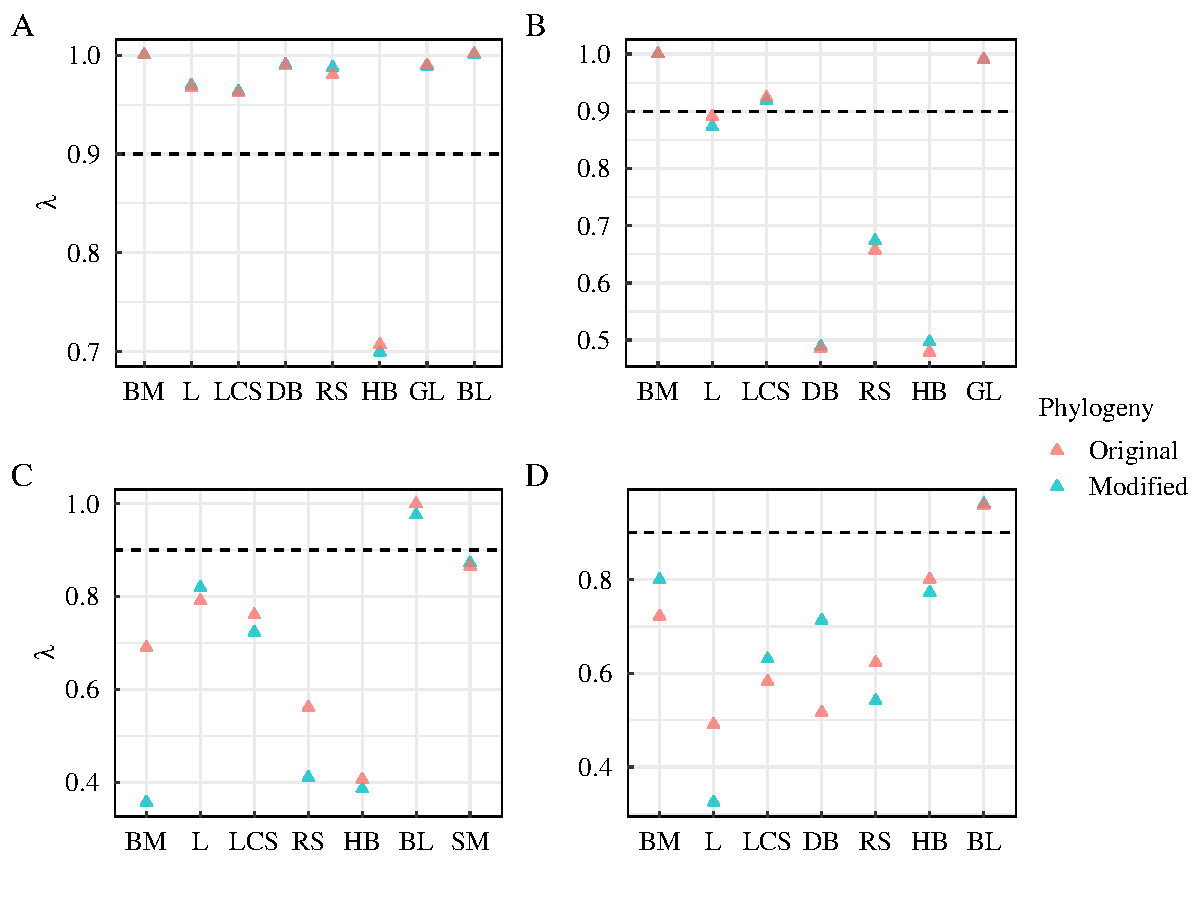
\includegraphics[scale=0.7]{figures/chapter2/Phylosignal/Continuous}
\caption[Phylogenetic signal in continuous traits(Pagel's $\lambda$) estimated with both original phylogenies and modified phylogenies]{\textbf{Phylogenetic signal in continuous traits(Pagel's $\lambda$) estimated with both original phylogenies and modified phylogenies.}}
\label{signalcontinuous}
\end{figure}

\begin{figure}[h!]
\centering
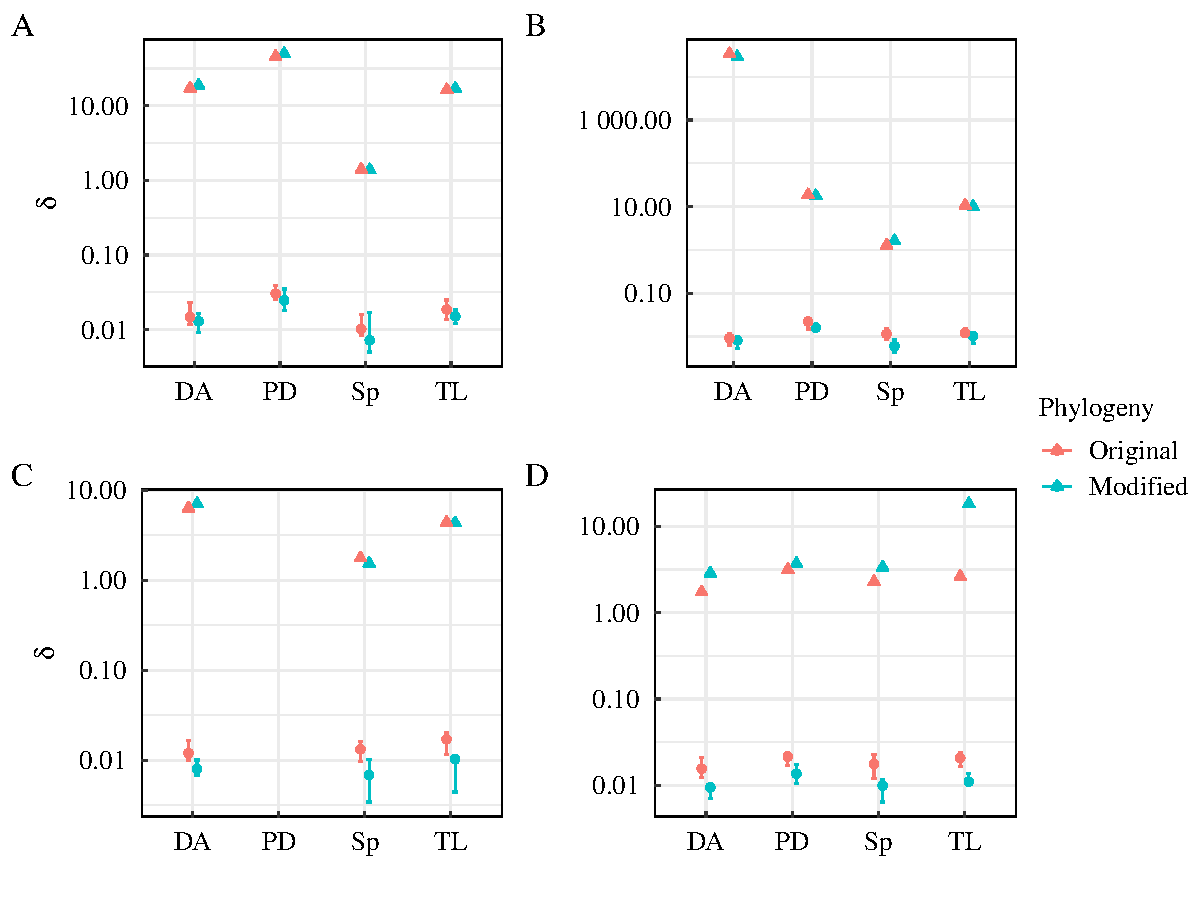
\includegraphics[scale=0.7]{figures/chapter2/Phylosignal/Categorical}
\caption[Phylogenetic signal in categorical traits ($\delta$) estimated with both original phylogenies and modified phylogenies]{\textbf{Phylogenetic signal in categorical traits ($\delta$) estimated with both original phylogenies and modified phylogenies.}}
\label{signalcontinuous}
\end{figure}

I hence imputed missing trait values using random forest algorithms, implemented by missForest. As stated above, missForest was shown by Penone et al (2014) to be the best method when including phylogenetic information for mixed-type variable imputations. Phylogenetic relationships were included as additional predictors in the form of phylogenetic eigenvectors, extracted from the phylogenies using the PVR package (Santos 2018). Penone et al (2014) also showed that including the first 10 eigenvectors minimised the imputation error. As not all species were represented in the phylogenies (Figure \ref{species_rep_phylo}), phylogenetic eigenvectors presented some missing values. I added taxonomic orders as a predictor variable. All traits in Figure \ref{traitcov} were included in the imputations, except for primary diet and diet breadth in reptiles.


\subsubsection{Imputation error and robustness}
To assess imputation accuracy, I used the `out-of-bag' error (OOB error) calculated by the missForest function. The missForest algorithm proceeds iteratively, training a random forest on observed values first, then predicting missing values over several iterations. When the difference between the last imputed dataset and the previous imputed dataset increases, the stopping criterion is met. The penultimate imputed dataset is then returned. For continuous variables, this difference, $\Delta_{cont}$,  is defined as:
\begin{align}
\Delta_{cont}=\frac{\sum_{j \in N}\left(X^{i,l}-X^{i,p}\right)^2}{\sum_{j \in N}\left(X^{i,l}\right)^2}, 
\end{align}
where $j$ is a continuous trait among $N$ traits, $X^{i,l}$ is the last imputed dataset and $X^{i,p}$ is the penultimate imputed dataset.  $\Delta_{cont}$ is a measure of the aggregated distance between two successive imputations on all continuous traits.  For categorical variables, the difference $\Delta_{cat}$ is:
\begin{align}
\Delta_{cat}=\frac{\sum_{k \in F}\sum_{j} J_{X^{i,l}\neq X^{i,p}}}{n(NA)}, 
\label{eqPFC}
\end{align}
where $k$ is a categorical trait among $F$ categorical traits, $n(NA)$ is a the number of missing values for $k$ and $J$ is the $j^{th}$ imputed values for which the consecutive imputations predicted contradicting results. In other words, $\Delta_{cat}$ measures the proportion of values that were found to be different between two successive imputations.
See Stekhoven (2011) for more details.

When the stopping criterion has been met, imputation error rates can be estimated. A mean square error (MSE) for each continuous trait and a proportion of falsely classified values (PFC) for each categorical trait are returned (the function can also return an overall normalised MSE for all continuous and overall PFC values for all categorical traits). The MSE for a trait is defined as:
\begin{align}
\sqrt{\frac{mean\left(\left(X_t-X_i\right)^2\right)}{var\left(X_t\right)}}, 
\end{align}
where $X_t$ is a vector of the complete trait values and $X_i$ a vector of the imputed trait values (Stekhoven 2011). For categorical traits, the  is calculated as the PFC ($\Delta_{cat}$, Equation \ref{eqPFC}). Imputation performance improves with decreasing error values.

I imputed 8 trait datasets for each class and plotted the MSE and PFC across all imputations. I then investigated whether imputations were robust examining whether values across imputations were congruent, or, on the other hand, showed a high variability.


\pagebreak
\section{Results}

\subsection{Outputs}
I collected and imputed data for 10 traits across 11637 avian species, 5502 mammalian species, 10334 reptilian species and 6904 amphibian species. Datasets recording species accepted and synonymic binomial names are available alongside the trait data. 

\subsection{Biases in the availability of trait information: non randomness in coverage and completeness and patterns in missing trait values}

\subsubsection{Increases in coverage and completeness due to taxonomic corrections.} 
Figure \ref{traitcov} shows the trait coverage within each class and for each trait, before and after correcting for taxonomy. Figure \ref{traitcomp} shows the distribution of trait completeness before and after taxonomic corrections, as well as the median trait completeness for each class.
Across all classes, correcting for taxonomy increased trait coverage (Figure \ref{traitcov}). Nevertheless, the increase in coverage for reptiles was marginal, which may indicate that the procedure developed to extract and identify accepted names overall performed less well for reptilian species than for mammals, birds and amphibians. Similarly, correcting for taxonomy improved trait completeness in all classes (Figure \ref{traitcomp}). Wilcoxon rank sum tests, testing the null hypothesis that uncorrected and corrected completeness distributions came from the same population, rejected this hypothesis across all classes (alternative hypothesis: uncorrected medians were lower than corrected medians; mammals: p-value=1.2$\cdot10^{-9}$; birds: p-value<2.2$\cdot10^{-16}$; reptiles: p-value=0.025; amphibians: p-value<2.2$\cdot10^{-16}$). To conclude, correcting for taxonomy had a significant impact on trait completeness and increased coverage in most cases. 

\subsubsection{Among-class biases in the availability of trait information}

\paragraph{Trait coverage.}
Trait coverage was highly variable across classes and traits. Trait coverage was initially good for most mammalian and avian traits, which had more than 50\% coverage (Figure \ref{traitcov} A and B). Only longevity had a coverage lower than 50\% for these classes, although generation length was above 80\% in both cases. Conversely, trait coverage was overall much poorer for reptiles and amphibians (Figure \ref{traitcov} C and D). About two-thirds of amphibian and reptilian traits presented a coverage below 50\%.  Amphibians and reptiles appeared to be less sampled in all traits, except in body mass (reptiles) and in body length, range size and habitat variables (amphibians).  As such, contrasting patterns of trait coverage appeared between, on the one hand, mammals and birds, and on the other hand, amphibians and reptiles. For species found in PREDICTS only, coverage increased disproportionally in reptiles and amphibians compared to the coverage for the full set of species (the figure for PREDICTS species only is available in the SI).

\begin{figure}[h!]
\centering
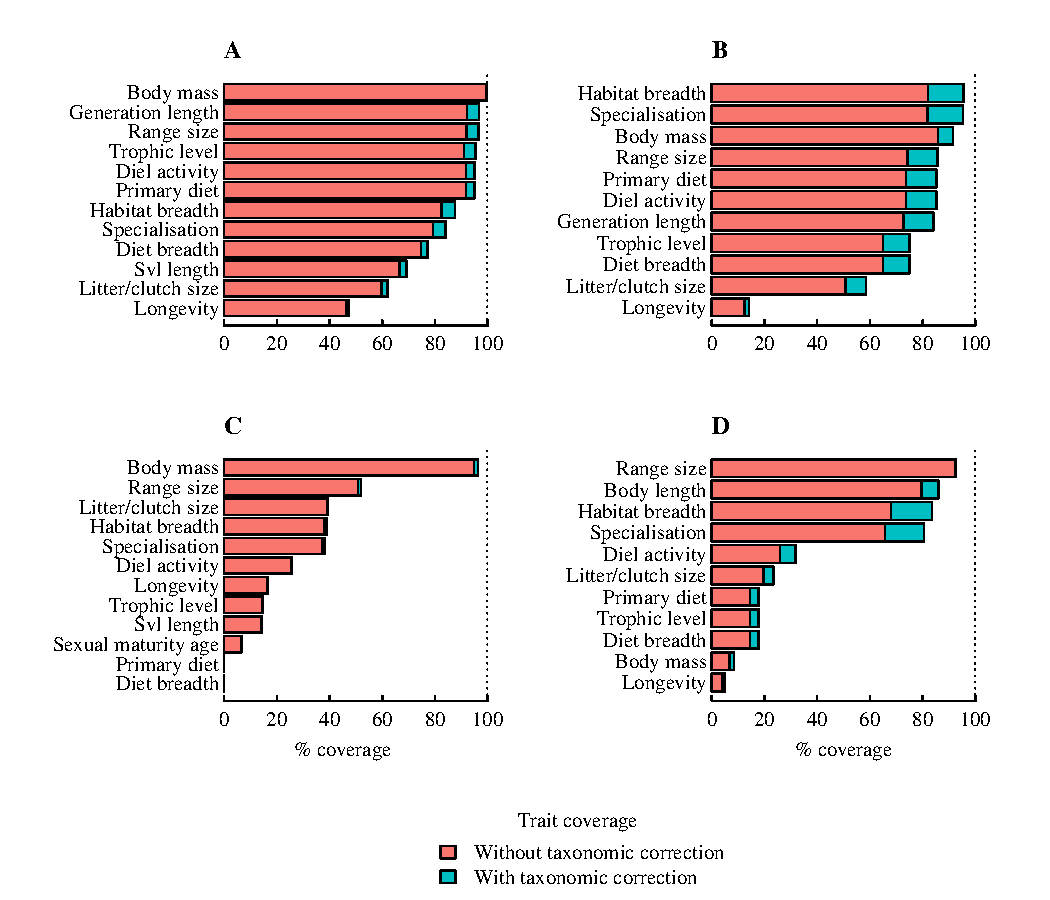
\includegraphics[scale=0.85]{figures/chapter2/Trait_coverage/Predictor_traits/All_species}
\caption[Trait coverage across all species before and after taxonomic correction]{\textbf{Trait coverage across all species before and after taxonomic correction.} Here are shown all targeted traits as well as a few other traits used in imputations, as additional predictors (such as generation length for mammals and birds or body length for amphibians). \textbf{(A)} Mammals (5885 species before correction, 5502 and after correction); \textbf{(B)} birds (13554 species before correction, 11637 after correction); \textbf{(C)} reptiles (10722 species before correction, 10334 after correction) and \textbf{(D)}; coverage across amphibians (8643 species before correction, 6904 after correction). Trait coverage was calculated as the percentage of species for which trait information was available. Correcting for taxonomic synonymy improved coverage in most cases. For mammals and birds, all traits had an initial coverage of more than 50\%, except longevity (but generation lengths were estimated for most species). On the other hand, trait coverage was poor (below 50\%) for about two thirds of collected reptilian and amphibian traits. A clear contrast in trait information appeared between mammals and birds versus amphibians and reptiles, highlighting the existence of important taxonomic biases in data collection.}
\label{traitcov}
\end{figure}

\paragraph{Trait completeness.}
Trait coverage revealed taxonomic biases, with higher resolution of trait information across mammals and birds. Trait completeness reflected similar biases. (Figure \ref{traitcomp}). The median completeness with taxonomic correction was high for mammals and birds (92\% and 82\% respectively) but much lower for reptiles and amphibians (30\% and 36\% respectively). A pairwise Kruskall-Wallis rank sum test rejected the hypothesis that completeness distribution across classes originated from the same distribution (p-values<2$\cdot10^{-16}$ in all cases), showing that class had a significant effect on the availability of trait information. 

\begin{figure}[h!]
\centering
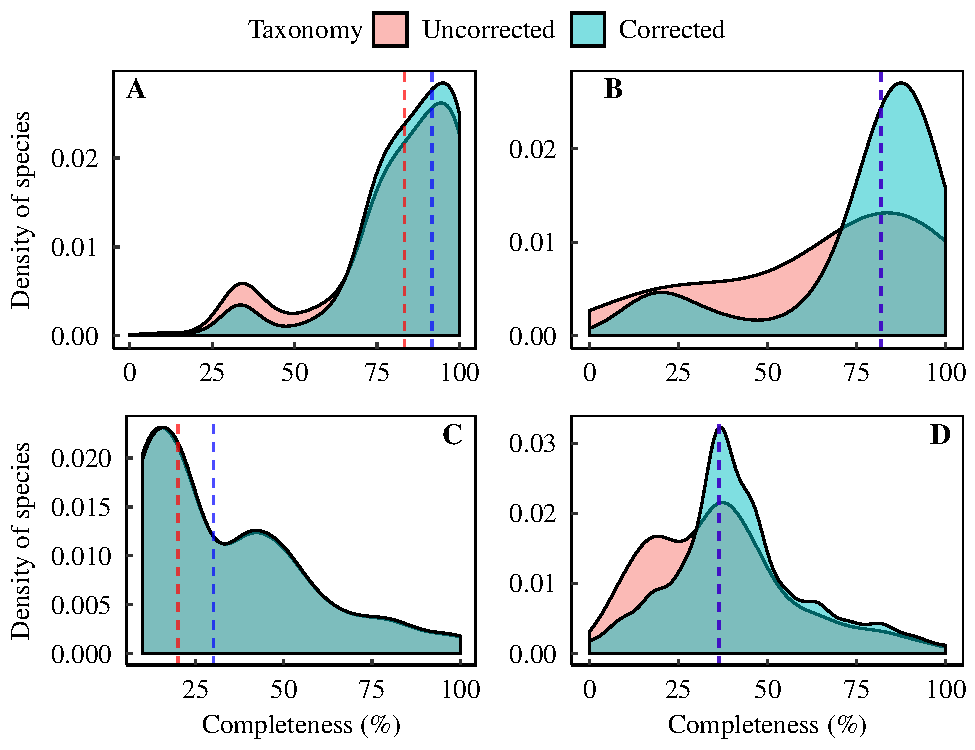
\includegraphics[scale=0.70]{figures/chapter2/Trait_coverage/Missing_values/Traitcompleteness}
\caption[Distribution of completeness of trait information across species]{\textbf{Distribution of completeness of trait information across species.} \textbf{(A)} Mammals; \textbf{(B)} birds; \textbf{(C)} reptiles and \textbf{(D)} amphibians. Completeness was calculated here for the same set of traits shown in Figure \ref{traitcov} (all predictor traits). Correcting for taxonomy affected completeness, significantly shifting the distributions to the right (alternative hypothesis, Wilcoxon rank sum tests: uncorrected medians were lower than corrected medians; mammals: p-value=1.2$\cdot10^{-9}$; birds: p-value<2.2$\cdot10^{-16}$; reptiles: p-value=0.025; amphibians: p-value<2.2$\cdot10^{-16}$). Class had a significant effect on median trait completeness (a pairwise Kruskall-Wallis rank sum test rejected the null hypothesis that completeness distributions across classes originated from the same distribution (p-values<$2\cdot10^{-16}$ in all cases)).}
\label{traitcomp}
\end{figure}

\subsubsection{Non-randomness in trait information availability within classes: patterns of missing trait values with regards to phylogenies}
Beyond cross-class biases in the availability of trait information, within-class patterns of missing values showed that certain families were less sampled than others.

\paragraph{Within-class patterns of trait coverage}

\pagebreak

% Mammals
\begin{figure}[h!]
\centering
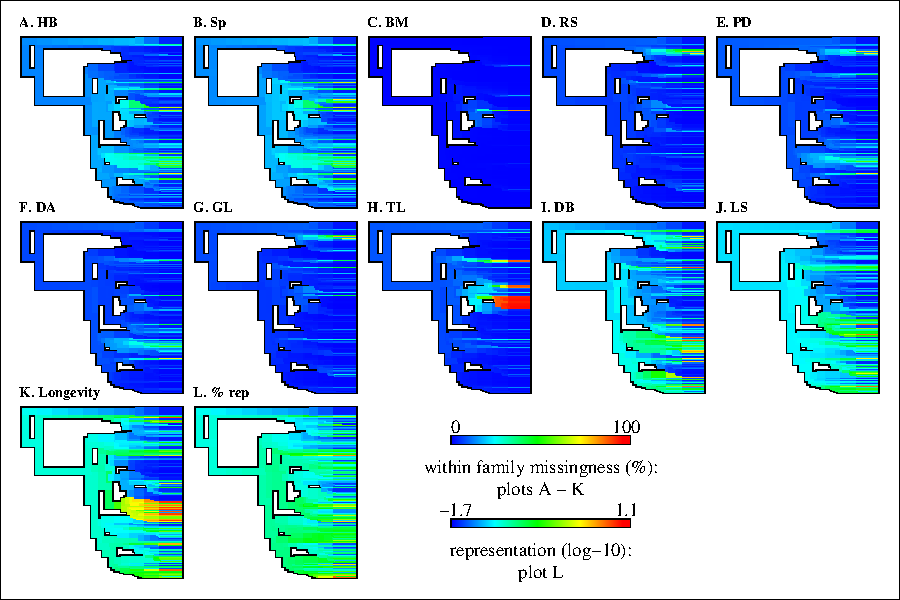
\includegraphics[scale=1]{figures/chapter2/NA_phylo_patterns/Mammals_coverage}
\caption[]{{}}
\label{familycov_mammals}
\end{figure}

% Birds
\begin{figure}[h!]
\centering
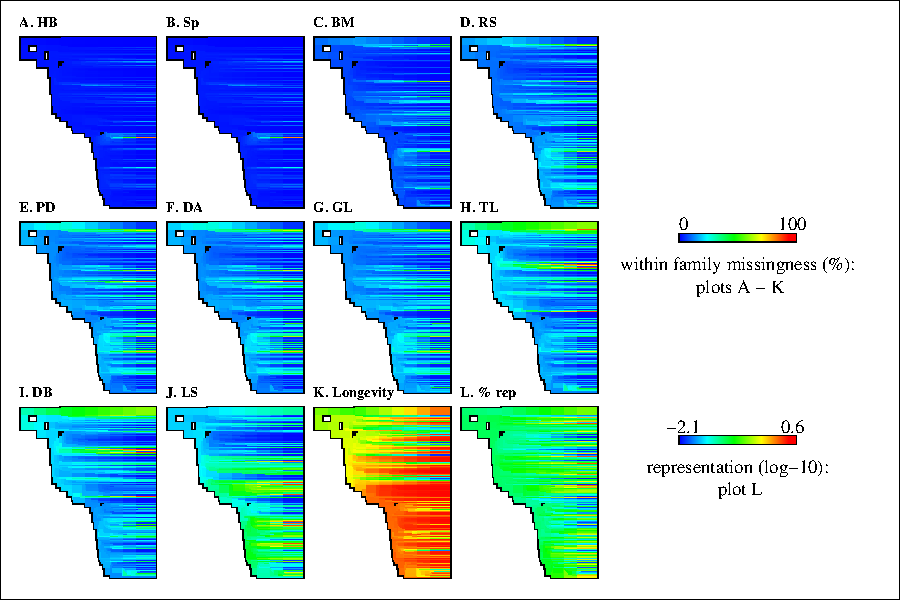
\includegraphics[scale=1]{figures/chapter2/NA_phylo_patterns/Birds_coverage}
\caption[]{{}}
\label{familycov_birds}
\end{figure}

\pagebreak

% Reptiles
\begin{figure}[h!]
\centering
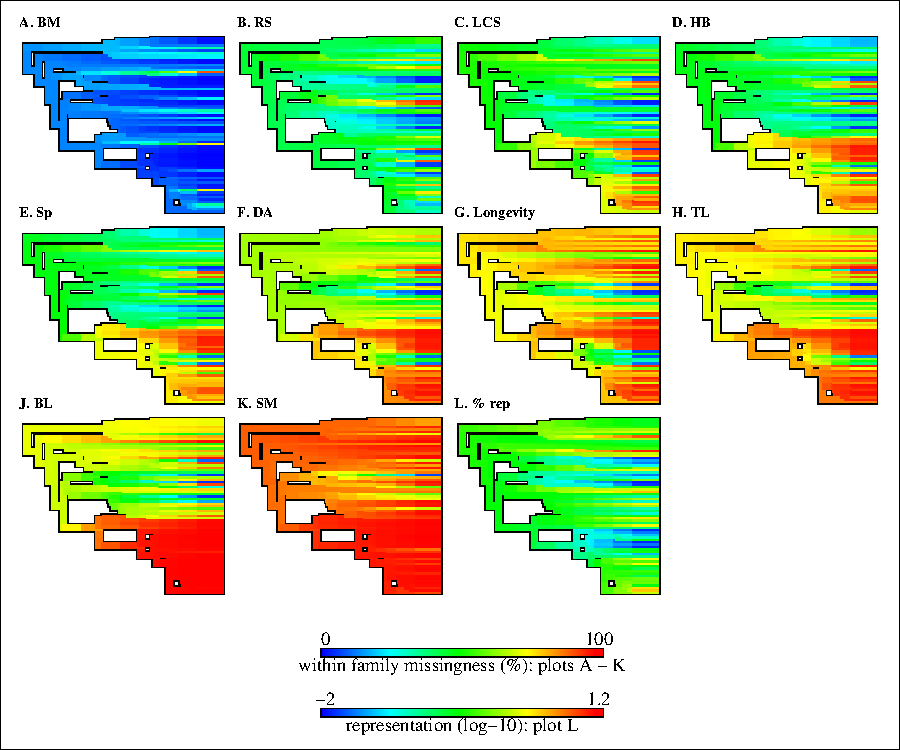
\includegraphics[scale=0.9]{figures/chapter2/NA_phylo_patterns/Reptiles_coverage}
\caption[]{{}}
\label{familycov_reptiles}
\end{figure}

% Amphibians
\begin{figure}[h!]
\centering
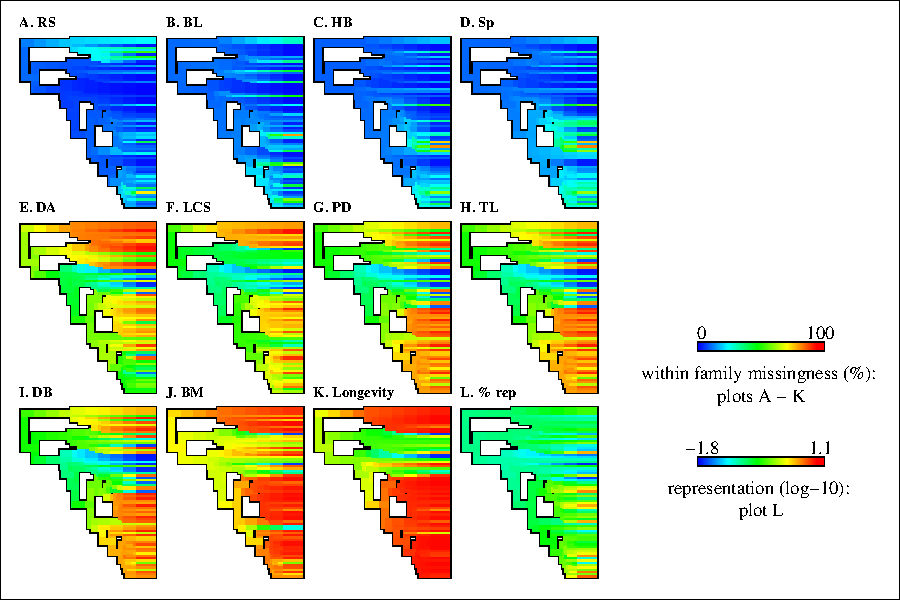
\includegraphics[scale=0.9]{figures/chapter2/NA_phylo_patterns/Amphibians_coverage}
\caption[]{{}}
\label{familycov_amphibians}
\end{figure}


\pagebreak

\paragraph{Within-class patterns of trait completeness}


\begin{figure}[h!]
\centering
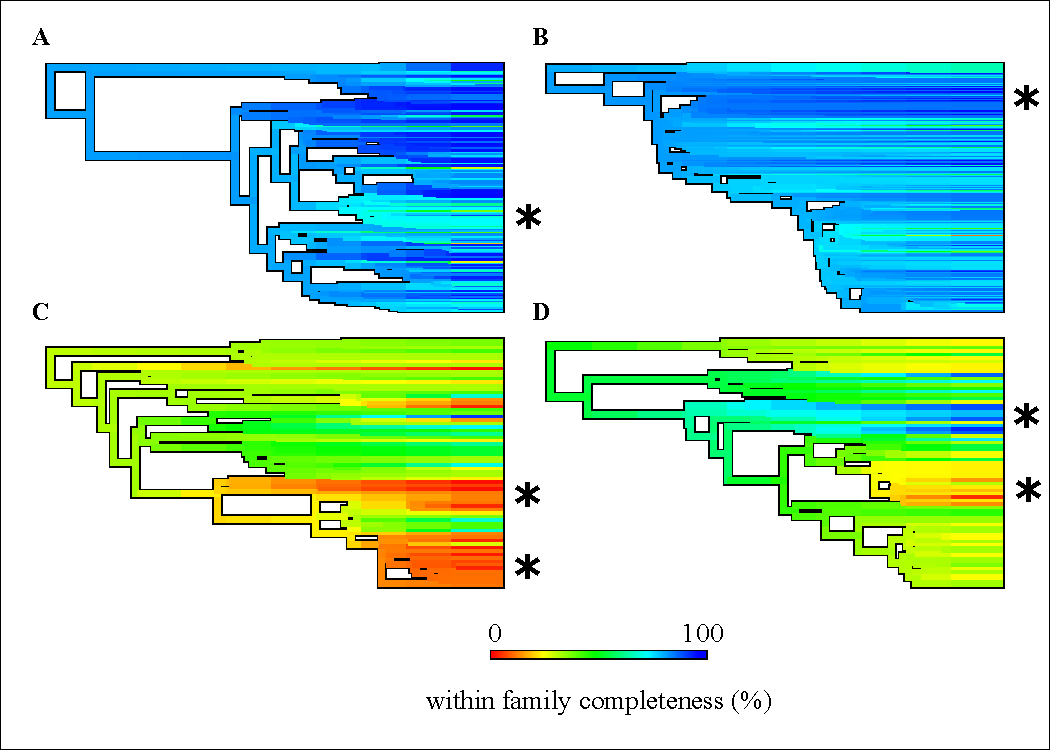
\includegraphics[scale=0.75]{figures/chapter2/NA_phylo_patterns/Completeness_all}
\caption[Median completeness across families]{\textbf{Median completeness across families.} Tips labels are not shown here for better visualisation of the results; the same figures with tip labels are provided in the SI (zooming into the figure is necessary for mammals and birds); tip label information includes order and family. \textbf{(A)} Mammalian family tree; \textbf{(B)} avian family tree; \textbf{(C)} reptilian family tree and \textbf{(D)} amphibian family tree. Median trait completeness was calculated within families and colour-coded  against tree branches.}
\label{classcomp}
\end{figure}

\subsection{Imputation performance and robustness}

\subsubsection{Out-of-bag imputation errors}

\begin{figure}[h!]
\centering
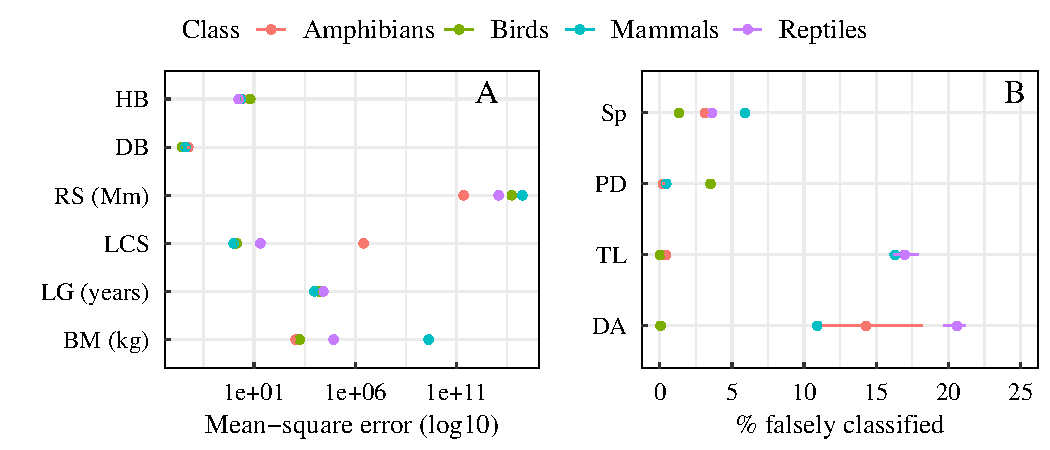
\includegraphics[scale=0.75]{figures/chapter2/Imputation_errors/MSE_PFC}
\caption[missForest mean-square errors and proportion of falsely classified values]{\textbf{missForest mean-square errors and proportion of falsely classified values.} \textbf{(A)} Mean-square errors for continuous traits. \textbf{(B)} Proportion of falsely classified values.}
\label{plotPFC}
\end{figure}

\subsubsection{Congruence of imputed values among 8 imputed datasets}

\begin{figure}[h!]
\centering
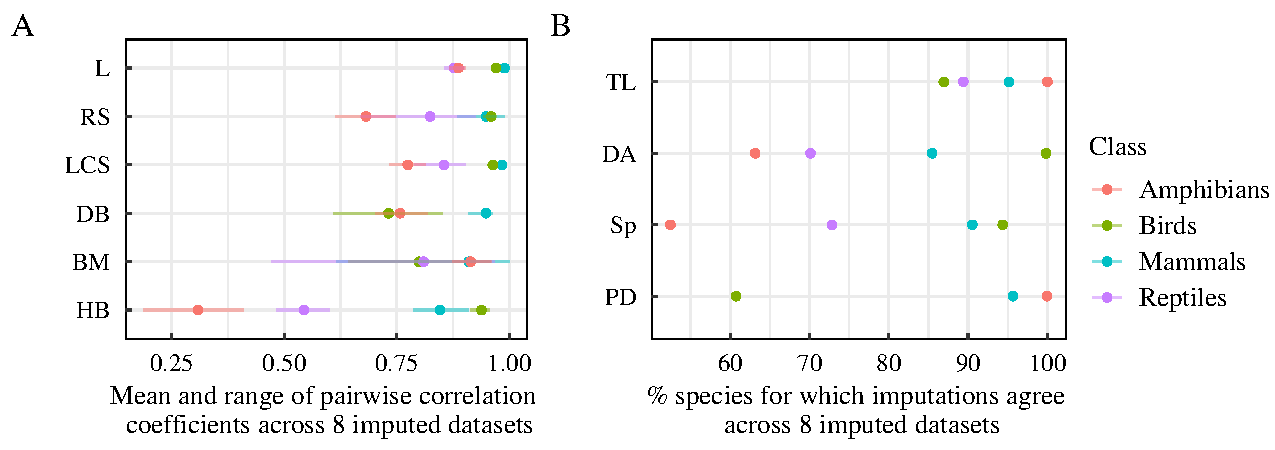
\includegraphics[scale=0.75]{figures/chapter2/Congruence_imputations/Summary}
\caption[]{{}}
\label{plotPFC}
\end{figure}

\subsubsection{Comparison with another collected and imputed datasets for mammals and birds}

\pagebreak
\section{Discussion}
\begin{itemize}
\item Taxonomic challenges
\item Manipulation of the phylogenies
Adding species randomly => justified if traits have a strong phylogenetic signal even with the uncorrected phylogeny. Then adding species makes sense (because strong phylogenetic signal, "trade-off" between the quality of the imputations versus the quality of the phylogenies)
\item Biases in availability of trait information across classes, Raunkier shortfall
\item Imputation robustness 
\end{itemize}
% Finally, I discuss the weaknesses of the methodology
% Impossibility to get intra-specific variation.

Completeness is likely to have an important effect on trait imputations, as it is a reflection of how many predictors have an estimate for a species.